\documentclass[a4paper]{article}
\usepackage[utf8]{inputenc}
\usepackage[T2A]{fontenc}
\usepackage[12pt]{extsizes}
\usepackage{pdfpages}

\usepackage[english,russian]{babel}
\usepackage[left=10mm, top=10mm, right=10mm, bottom=20mm, nohead, nofoot]{geometry}
\usepackage{amsmath,amsfonts,amssymb} % математический пакет
\headsep=10mm

\usepackage[most]{tcolorbox} % для управления цветом
% НАСТРОЙКИ
%теорема
\definecolor{theorem-color}{gray}{0.90} % уровень прозрачности (1 - максимум)
\newtcolorbox{htheorem}{colback=theorem-color,grow to right by=-4mm,grow to left by=-4mm,
    boxrule=0pt,boxsep=0pt,breakable} % настройки области с изменённым фоном

%определение
\definecolor{def-color}{gray}{0.98}
\newtcolorbox{definit}{colback=def-color,grow to right by=-4mm,grow to left by=-4mm,
    boxrule=0pt,boxsep=0pt,breakable} % настройки области с изменённым фоном

%доказательсвто теоремы
\definecolor{proof-color}{gray}{0.95} % уровень прозрачности (1 - максимум)
\newtcolorbox{hproof}{colback=proof-color,grow to right by=-1mm,grow to left by=-1mm,
    boxrule=0pt,boxsep=0pt,breakable} % настройки области с изменённым фоном

%замечания, следствия
\definecolor{consectary-color}{gray}{0.95} % уровень прозрачности (1 - максимум)
\newtcolorbox{cns}{colback=consectary-color,grow to right by=-4mm,grow to left by=-4mm,
    boxrule=0pt,boxsep=0pt,breakable} % настройки области с изменённым фоном



\usepackage{fancybox,fancyhdr}
\pagestyle{fancy}

\usepackage{hyperref}
\hypersetup{colorlinks=true, allcolors=[RGB]{010 090 200}} % цвет ссылок 
\newcommand{\lr}[1]{\left({#1}\right)} % команда для скобок

\author{Васильев Павел}
%\linespread{1}
\usepackage{amsmath}

\usepackage{graphicx}
\usepackage{ifpdf}
\ifpdf
\DeclareGraphicsRule{*}{mps}{*}{}
\fi
\usepackage{graphicx}
\usepackage{color}
\graphicspath{ {images/} }

%\renewcommand{\familydefault}{\sfdefault}

\begin{document}

\section*{Численное интегрирование}

Приближённо вычислить значение интеграла 
\[
\int_0^1 e^{x^2} dx
\]

с шагом $0.1, 0.05, 0.025$.
Для каждого метода и шага указать погрешность по Рунге.

\textbf{Некоторые обозначения:}

Пусть всего $m$ точек разбиения $\{ x_j \}_{j=1}^m$, $h:= \frac{b-a}{m-1}$ - шаг.

\[a = x_1 < x_2 < ... < x_{m-1} < x_m = b\]

\[x_{j+1} - x_j = h, j = 1, ..., m-1\]

Формула левых прямоугольников:
\[ \int_0^1 e^{x^2} dx \approx h \sum_{j=1}^{m-1} e^{{x_j}^2} \]

Формула средних прямоугольников:
\[ \int_0^1 e^{x^2} dx \approx  h \sum_{j=1}^{m-1} e^{{x_j + \frac{h}{2}}^2} \]

Формула Симпсона:
\[ \int_0^1 e^{x^2} dx \approx  \frac{h}{6} \sum_{j=1}^{m-1} \left( e^{{x_j}^2} + 4 e^{\left(x_j+\frac{h}{2}\right)^2} + e^{{x_{j+1}}^2} \right) \]

Оценка погрешности по Рунге $R_h$:

\[ R_h = \frac{2^p}{2^p-1} (S_{\frac{h}{2}} - S_h)\]

где $S_h$ - результат численного интегрирования по формуле с шагом $h$, $p$ - это некоторое положительное число (известно, что для левых и правых прямоугольников $p = 1$, для средних прямоугольников и трапеции $p = 2$, для $\frac{3}{8}$ и Симпсона $p=4$).



Я написал код на $Python$, который применяет перечисленные методы с нужным шагом и оценивает каждый метод и каждый шаг по Рунге.

Результаты вывода программы на $Python$ (более подробно вычисления можно посмотреть в приложенном файле)

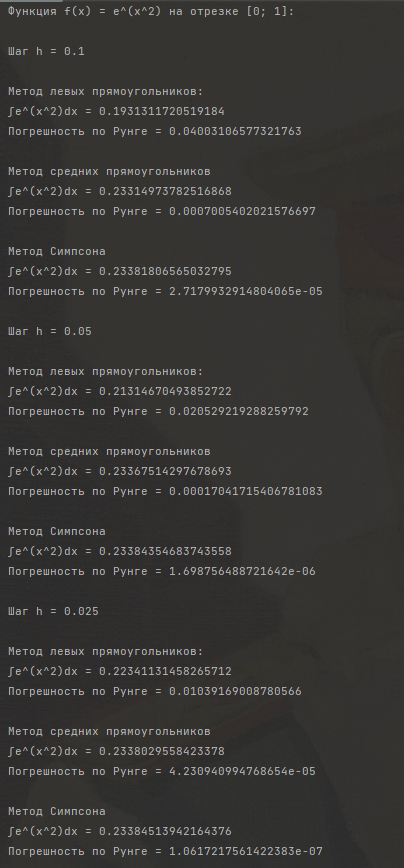
\includegraphics[scale=0.7]{results}

Из представленных результатов можно сделать вывод, что метод Симпсона дает наименьшую погрешность и наиболее точное значение интеграла по сравнению с методами левых прямоугольников и средних прямоугольников на всех трех значениях шага $h$.

Код:

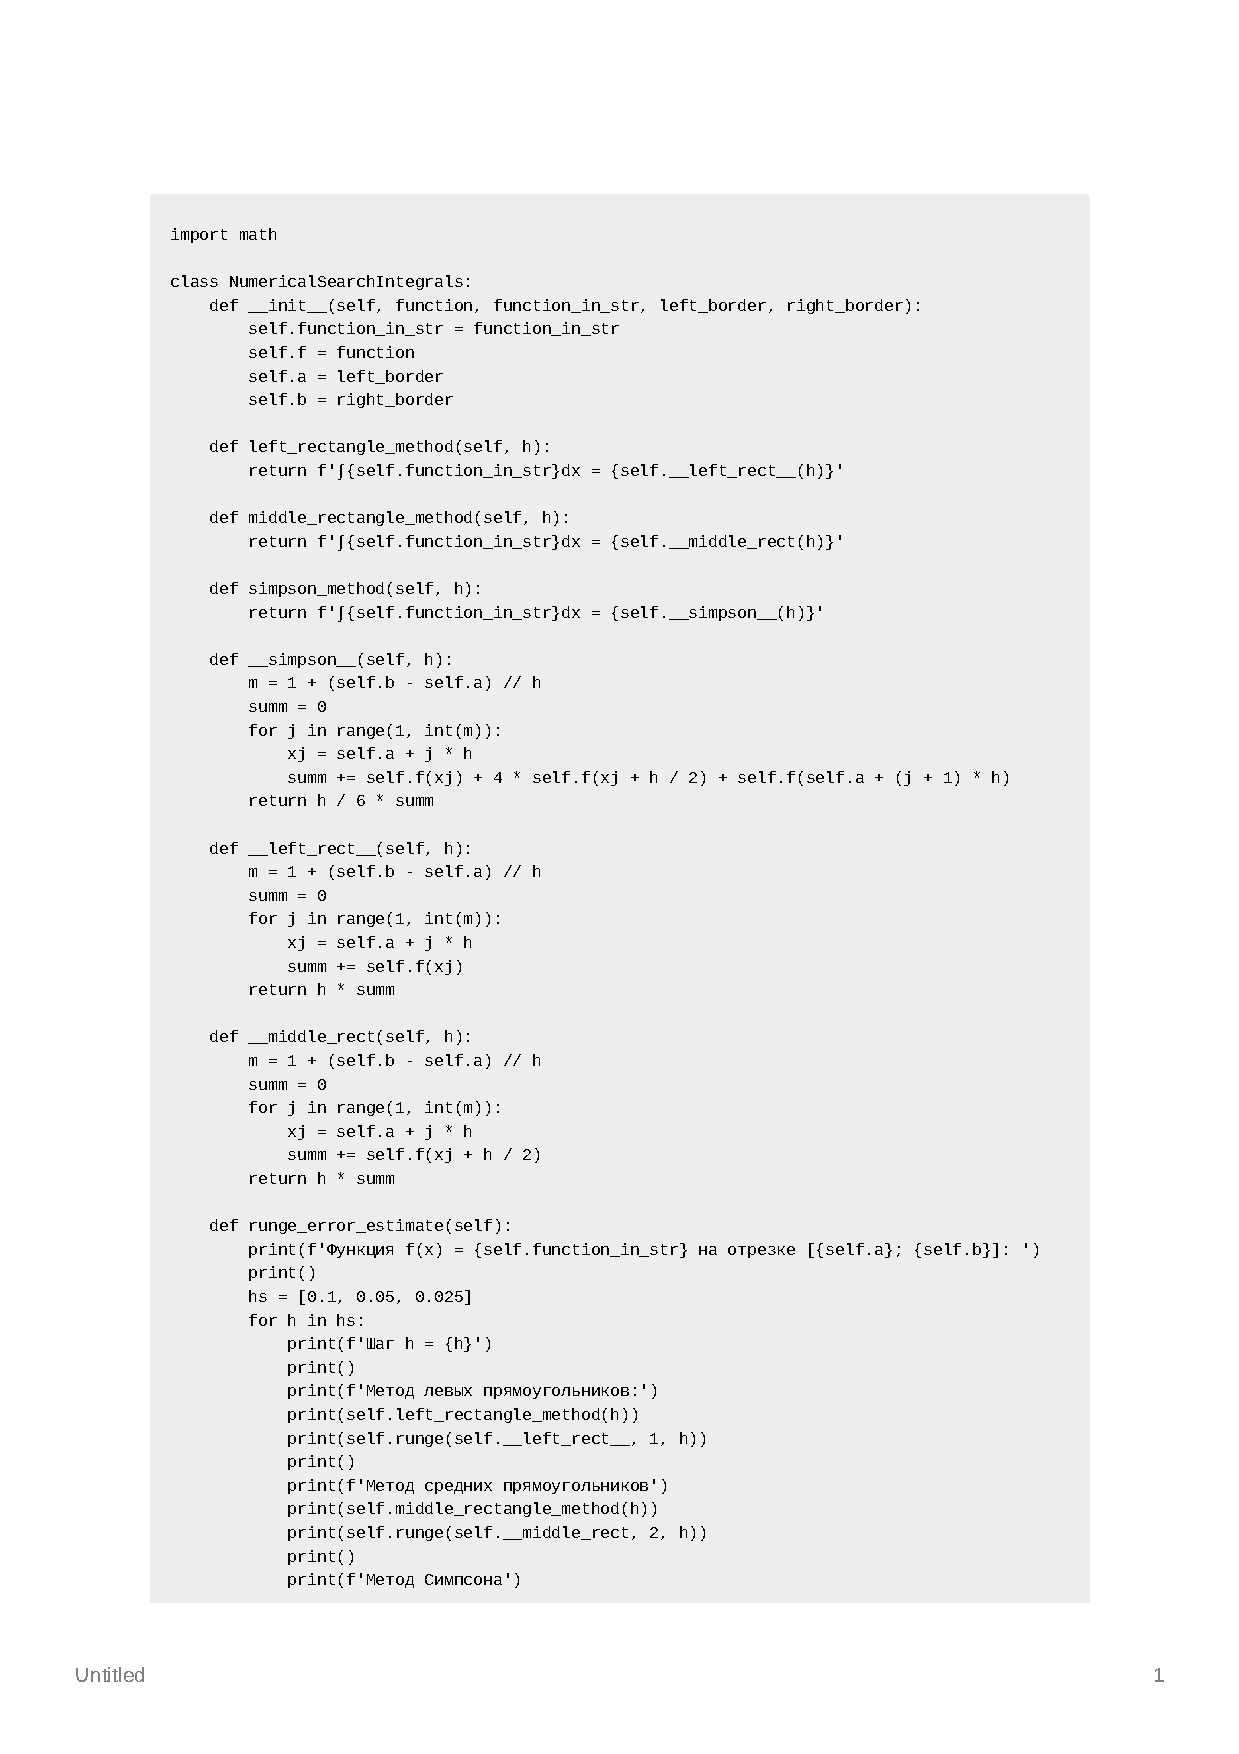
\includepdf[pages={1-}]{code.pdf} 

\end{document}